\documentclass[../main.tex]{subfiles}
\graphicspath{{\subfix{../figures/}}}

\begin{document}
\chapter{Evaluation and Conclusion} \label{chap:eval}

\section{Training Process and Random Validation} \label{sec:train_val}
In the end, our controller described in chapter \ref{chap:ctrl_design} is a combination of the following:
\begin{itemize}
    \item A six-element observation vector (Eq. \ref{eq:obs})
    \item A single scalar action of type $\mathtt{uint8}$ (Sec. \ref{sec:agent_action})
    \item Actor and critic networks of 256-node dense layers with ReLU activation (Sec. \ref{sec:agent})
    \item A hybrid reward function (Eq. \ref{eq:final_rwd}) and a realistic reset function (Eq. \ref{eq:resetfn})
\end{itemize}

Figure \ref{fig:training_result} depicts the learning progress of that setting against a second-order LTI plant (Eq. \ref{eq:narnia_sss}). In the first 50 episodes, the actor (dark blue plot) explores its state-action space by making random actions, hence negative returns. Next, it exploits those experiences to gradually improve until convergence around the $160^{th}$ episode. Later on, our agent keeps adding some Gaussian noise to its action for balancing with exploration, which occasionally causes a significant drop (e.g., episode $500^{th}$). This strategy enhances robustness to varying states. Simultaneously, the critic (orange plot) mirrors an upward trend, indicating an effective process. Consequently, they approach the same level as expected \cite{matlab_q0_support}.

Then, the finished model is assessed with a completely new initial state using another random seed. Note that our environment definition does not change. As a result, the regulator works perfectly (Fig. \ref{fig:val_result}).
\begin{figure}[htbp]
\centering
\begin{subfigure}{\textwidth}
    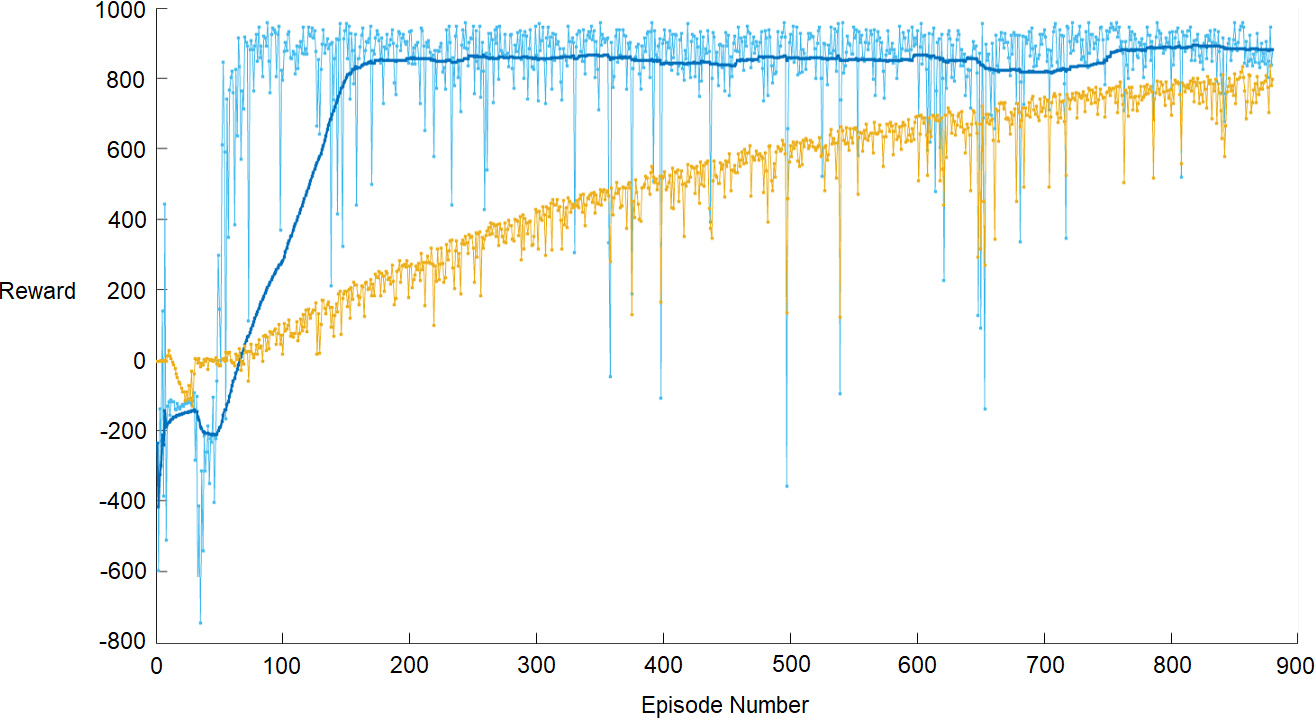
\includegraphics[width=\linewidth]{figures/final_result.png}
    \caption{Training process result}
    \label{fig:training_result}
\end{subfigure}
{}
\begin{subfigure}{\textwidth}
    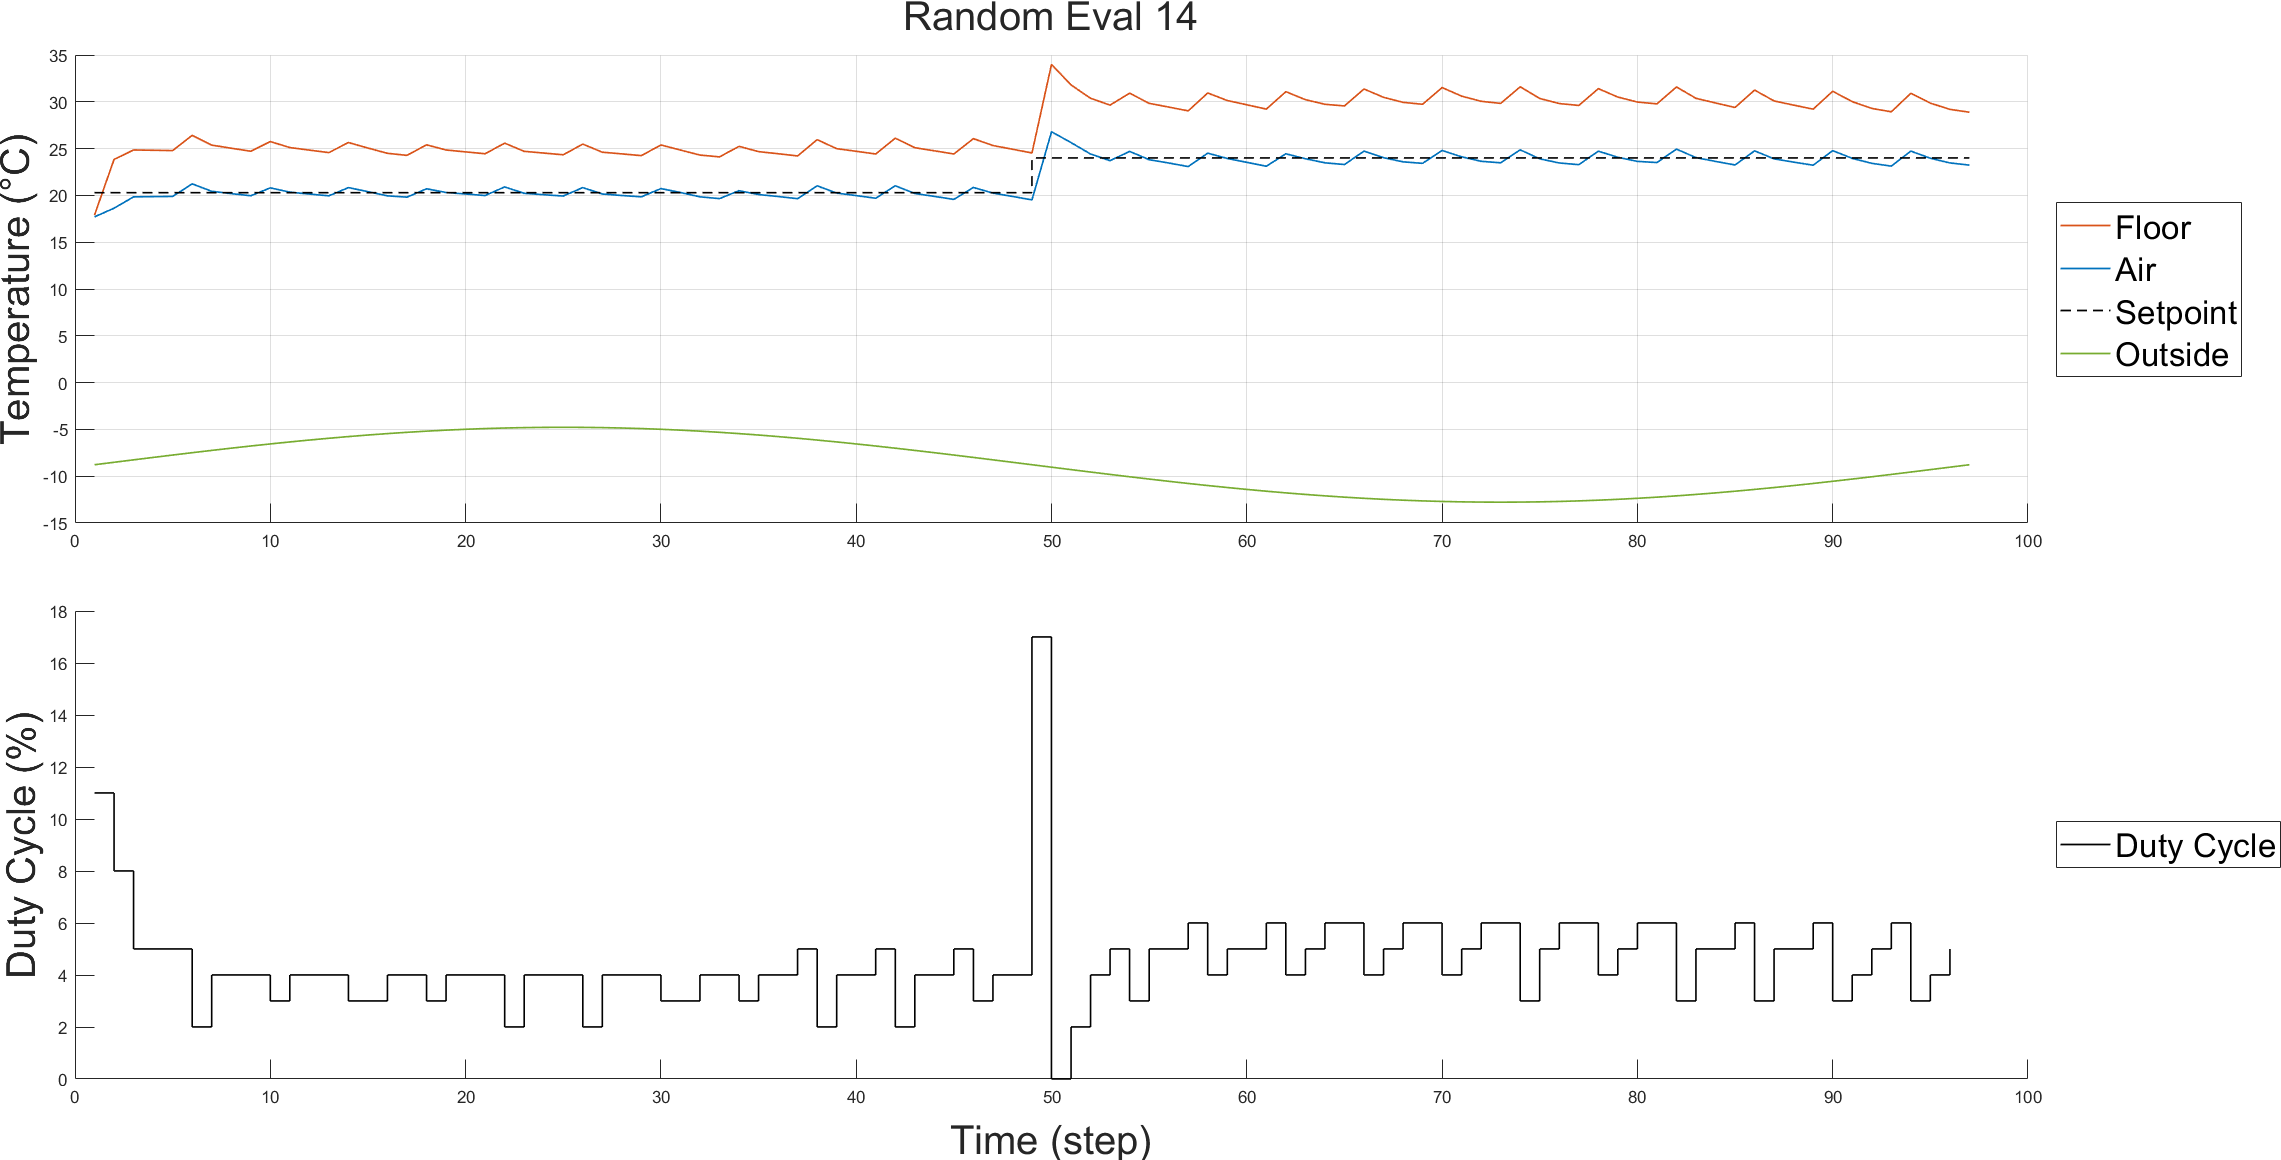
\includegraphics[width=1\linewidth]{figures/RandomEval14.png}
    \caption{Model outcome in a random case}
    \label{fig:val_result}
\end{subfigure}
\caption{Training and random validation results}
\label{fig:train_val}
\end{figure}


\section{Edge Cases}
In this section, we explore some edge cases the agent may not encounter during training. Statistically speaking, these samples are out of distribution (OOD). Due to the vast number of possible combinations, we only highlight a few notable cases. Keep in mind that they all use a two-ampere load unless noted otherwise. Since our focus here is on control stability, not comparison, certain metrics are omitted.

\nomenclature[D]{OOD}{Out-of-distribution samples that are not observed during a model's training process.}

\subsection{Cooling a Hot Room}
Section \ref{sec:train_val} proves that an RL agent works flawlessly in a heating task. Nonetheless, it should know when to pause, typically when starting from a higher degree, so that the room can cool down naturally to a desired setpoint. Figure \ref{fig:edge_1} visualizes an example in which initial floor and air temperatures are 28 (\degree C), whereas setpoints drop from 23 to 21 (\degree C). Fortunately, the controller operates well. 
\begin{figure}[htbp]
    \centering
    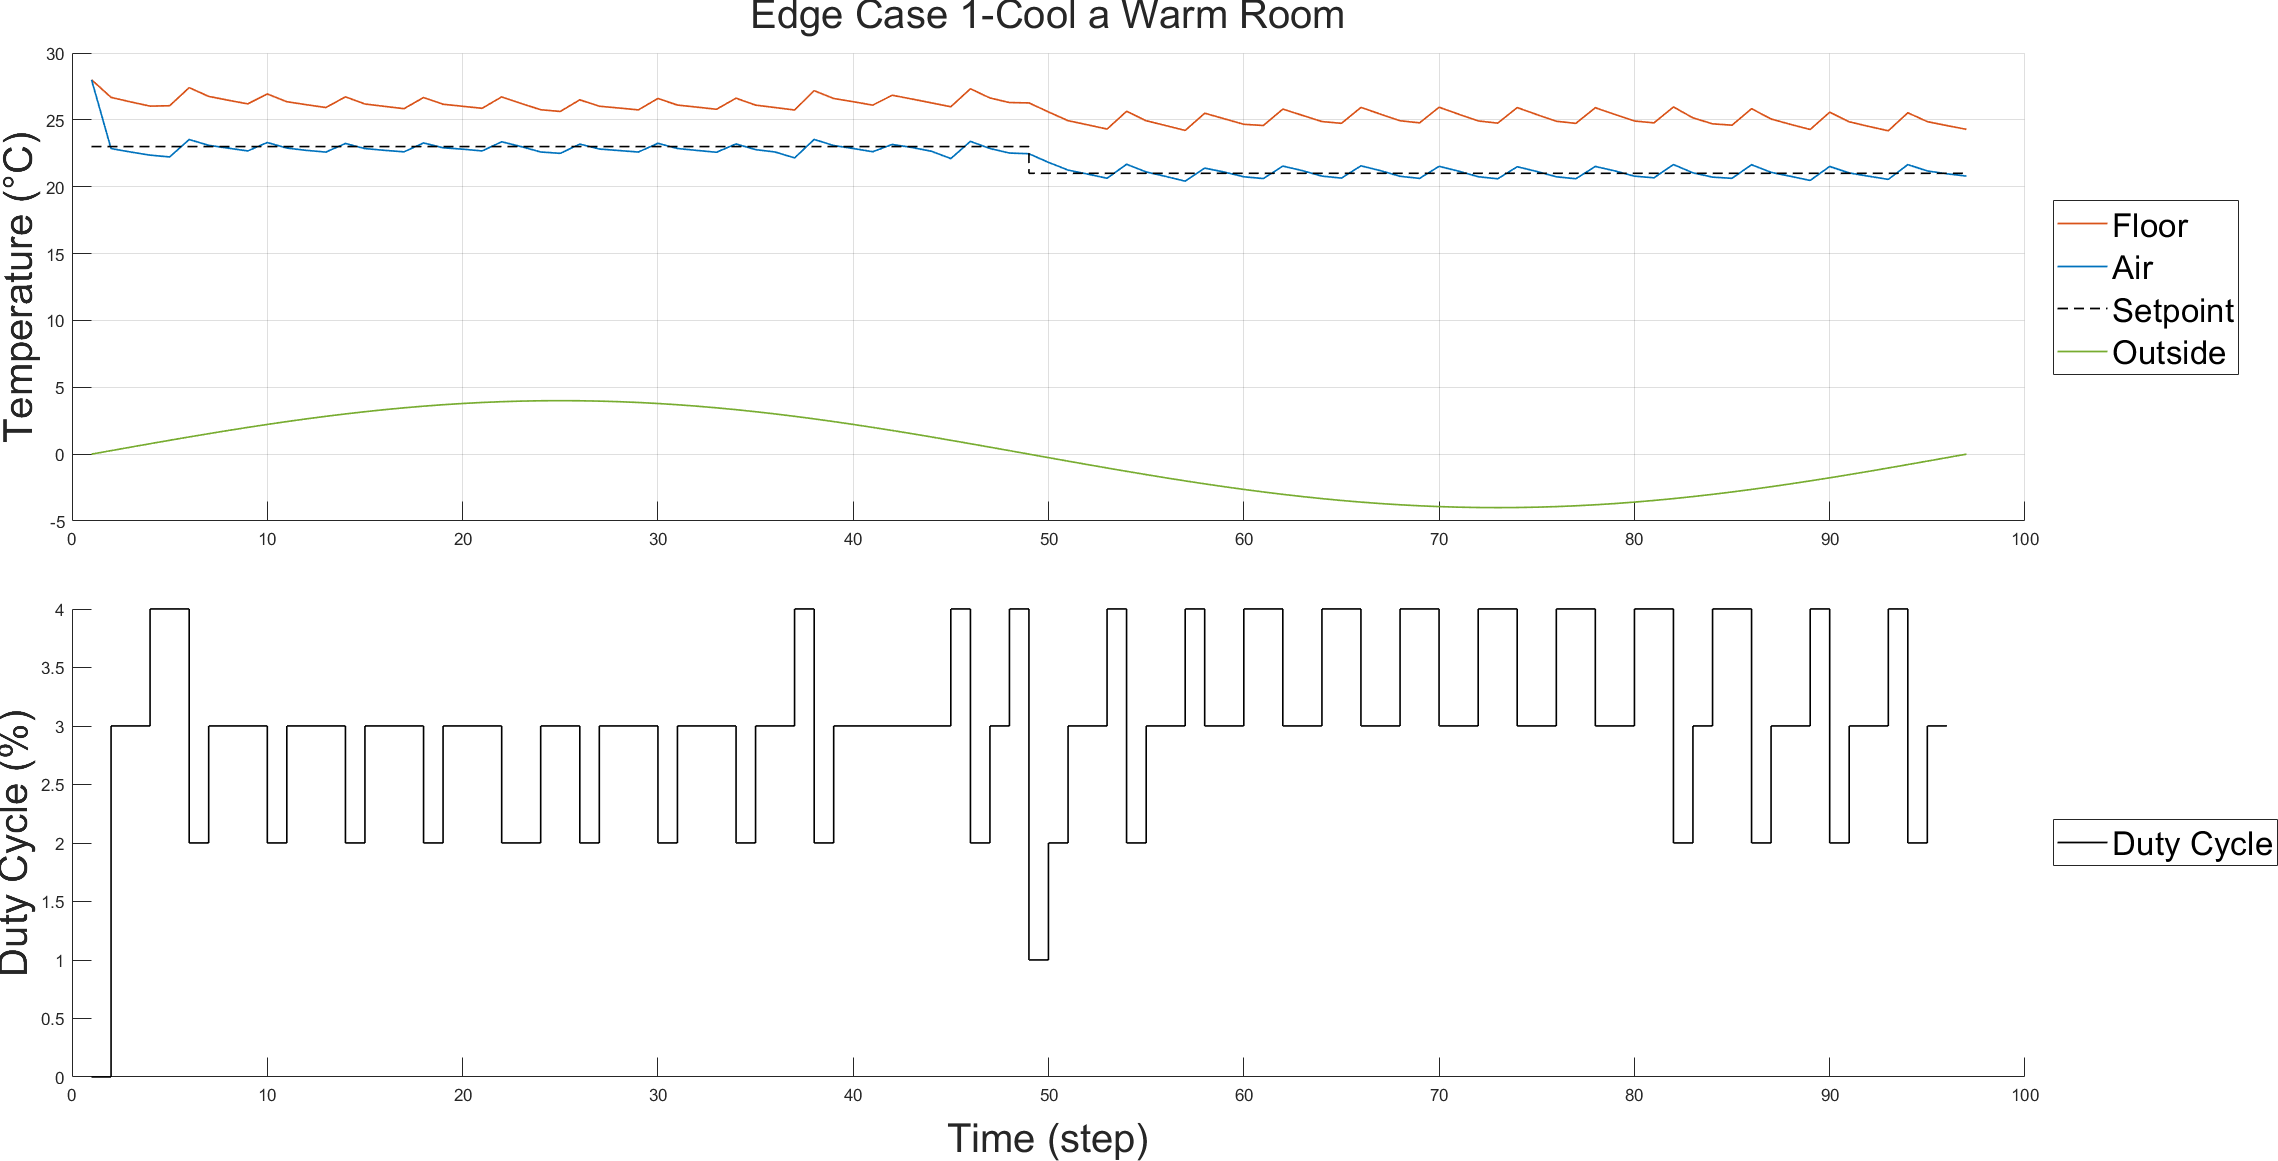
\includegraphics[width=1\linewidth]{figures/EdgeCase1-CoolaWarmRoom.png}
    \caption{Edge case 1: when it is too hot inside}
    \label{fig:edge_1}
\end{figure}

\subsection{Warm Weather Outside}
Similarly, when the exterior is warmer, heaters should turn off to save electricity. Instead, the room can rise to setpoints by absorbing the external thermal energy. In this example, a room must go from 19.5 to 21 (\degree C), given that it may get 1 (\degree C) hotter outside. Figure \ref{fig:edge_2} shows that our agent can cope with this situation. According to equation \ref{eq:pi}, a PI controller cannot do the same here as they always turn on if the error is positive and the floor is not overbounded.
\begin{figure}[htbp]
    \centering
    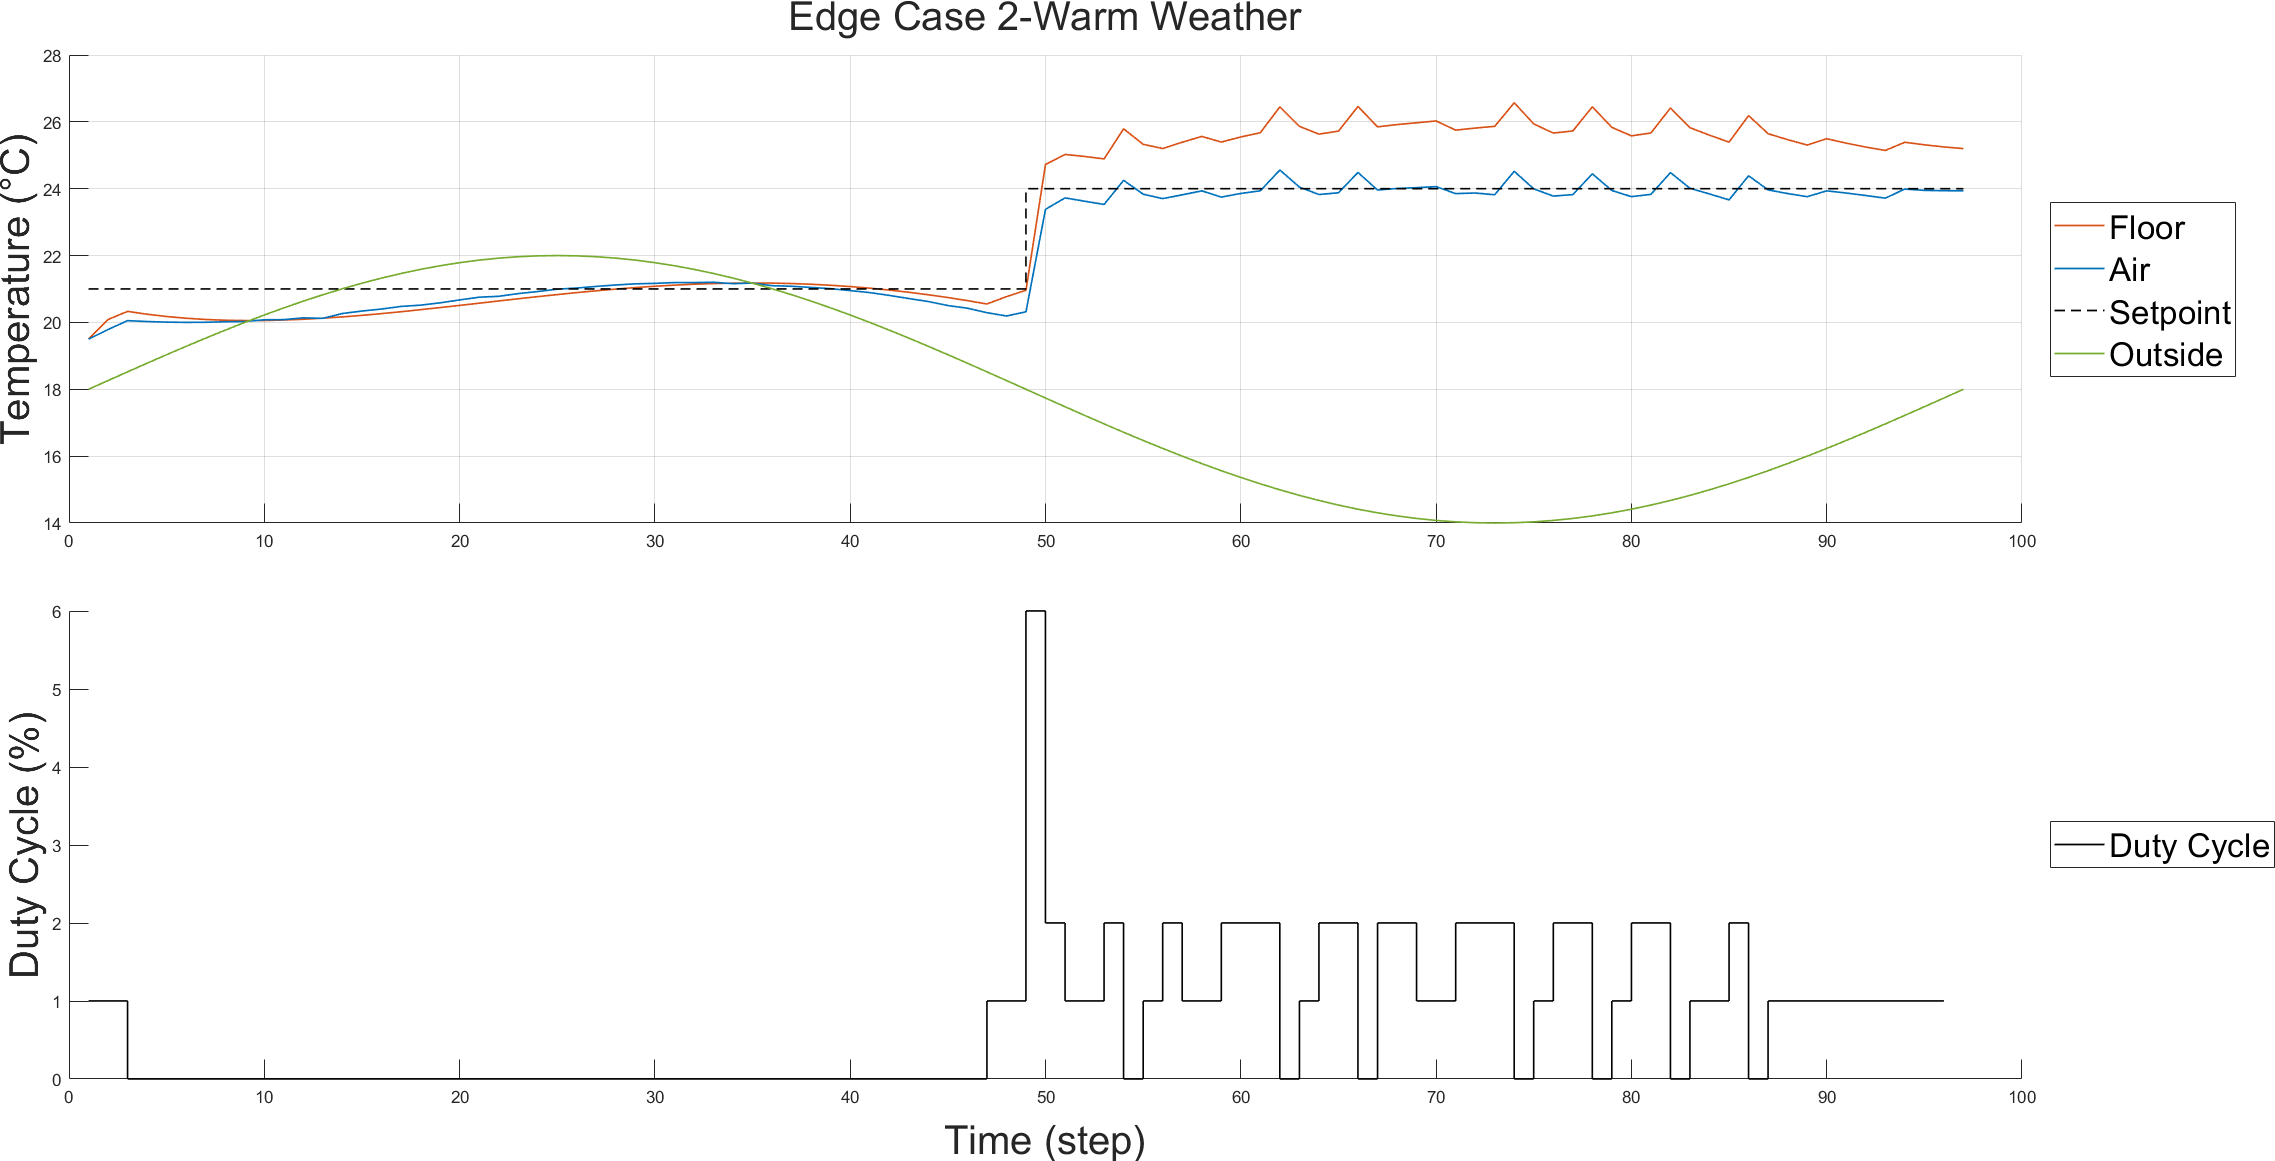
\includegraphics[width=1\linewidth]{figures/EdgeCase2-WarmWeather.png}
    \caption{Edge case 2: when the weather gets warm}
    \label{fig:edge_2}
\end{figure}

\subsection{Additive Immeasurable Disturbance}
In reality, a floor is usually warmer than air. Although we observe that in section \ref{sec:env_baseline}, it is not compulsory in simulation. For instance, when many people suddenly arrive in a 
meeting room of 10 (\degree C), the air jumps to 18.8 (\degree C at step $0^{th}$) or 31.14 (\degree C at step $61^{st}$). This is one type of immeasurable disturbance for which a controller must compensate. Indeed, after only one step (15 minutes), the room is back to the desired tolerance ($20.29 \pm 1.00$ \degree C), regardless that it is only -1 (\degree C) outside. (Fig. \ref{fig:edge_3}).
\begin{figure}[htbp]
    \centering
    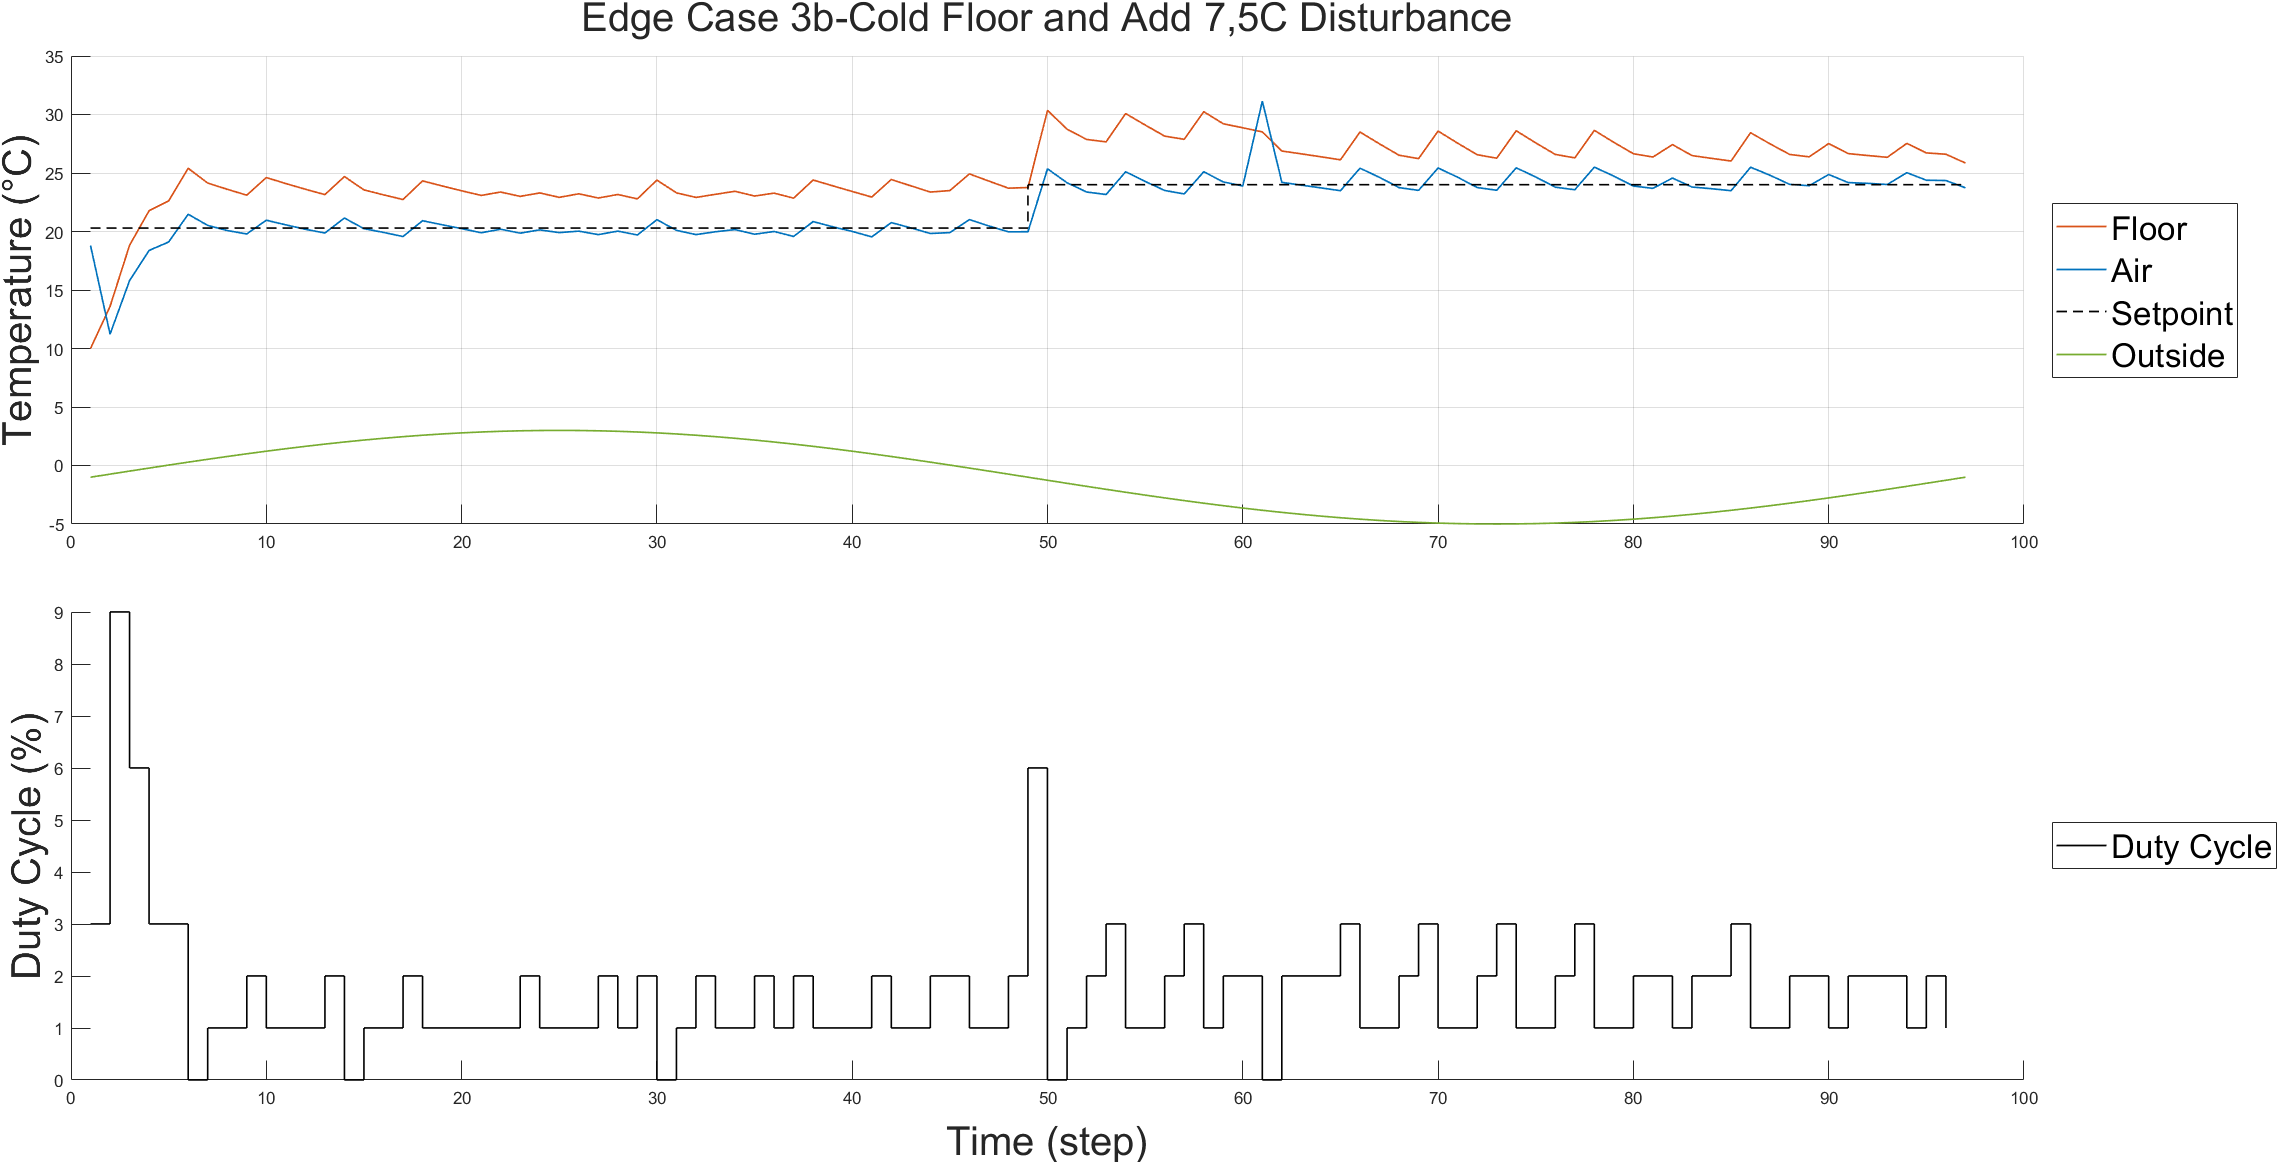
\includegraphics[width=1\linewidth]{figures/EdgeCase3b-ColdFloorandAdd7,5CDisturbance.png}
    \caption{Edge case 3: when many people suddenly appear}
    \label{fig:edge_3}
\end{figure}

\subsection{Start with a Nearly Overheated Floor}
Another interesting scenario occurs when the floor temperature is just below safety limits while the air temperature is far below setpoints. Here, we aim to increase a room from 15 to 20.29 (\degree C) with an exterior of 10 (\degree C). Our agent correctly handles this case by shutting down the system to make use of the residual heat. Although there is a slight performance dip between steps 30 and 40 with an error of 1.2 (\degree C), our agent might still outperform a traditional PI controller. In fact, a PI controller, in contrast, would activate the relay only to have it subsequently shut down by another safety mechanism.
\begin{figure}[htbp]
    \centering
    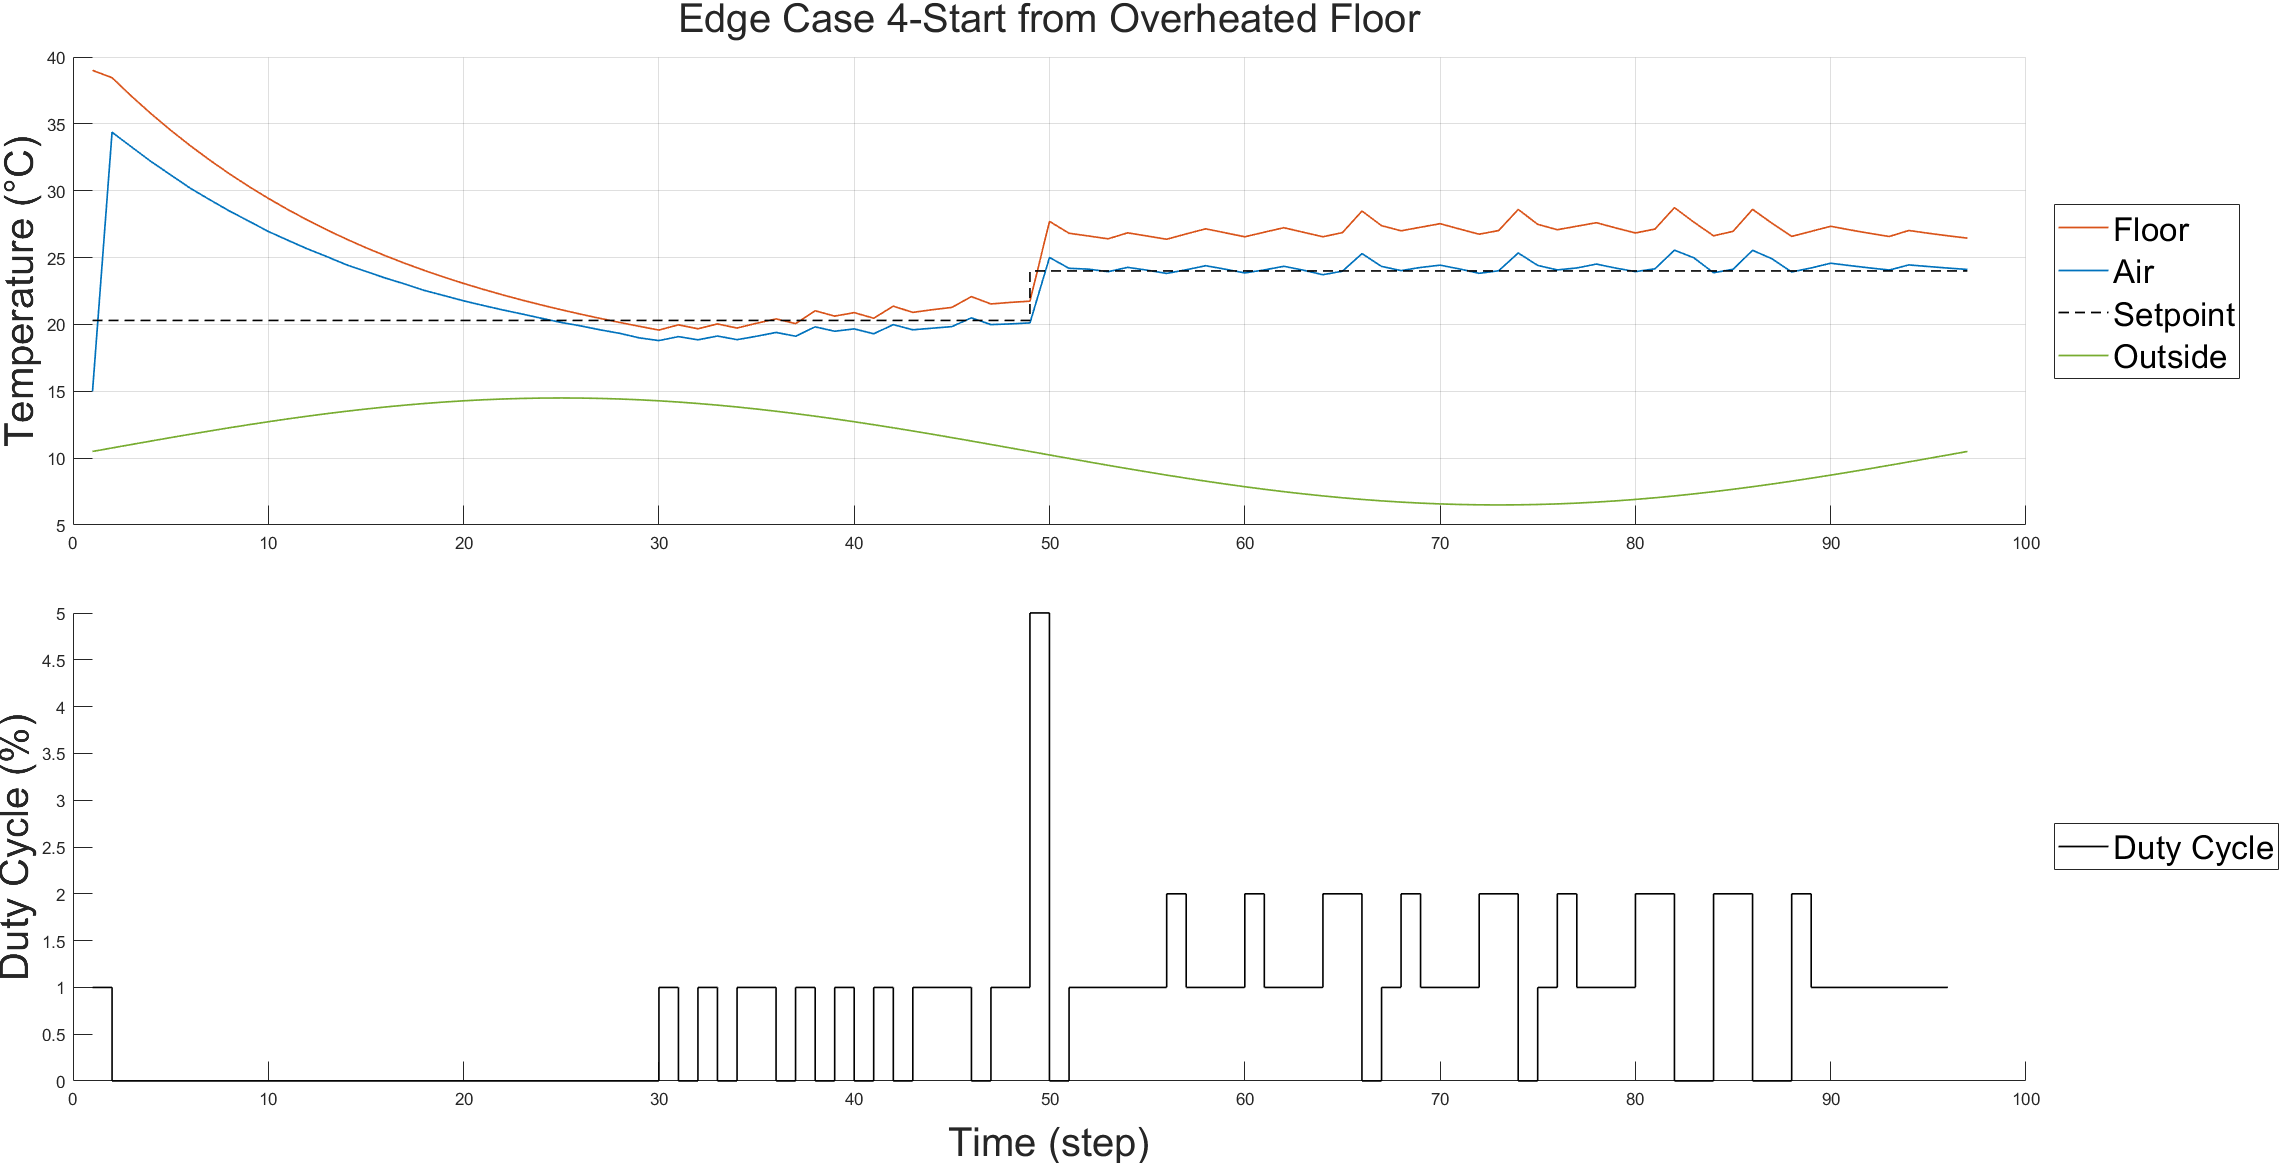
\includegraphics[width=1\linewidth]{figures/EdgeCase4-StartfromOverheatedFloor.png}
    \caption{Edge case 4: when a floor is close to limits}
    \label{fig:edge_4}
\end{figure}

\subsection{Quadruple Room Size}
So far, we have seen that a TD3-based controller is robust to a wide range of disturbances and starting points (extrinsic dynamical variation). However, given the same parameters in section \ref{sec:train_val}, when we quadruple the air and floor volume, i.e., by doubling width and depth (intrinsic dynamical variation), the agent no longer works (\ref{fig:edge_5a}). Intuitively, a bigger room needs a bigger load, so we doubled the input current, i.e., four times more power supply. Still, it became even worse (Fig. \ref{fig:edge_5b}). In fact, it completely shuts down with a belief that any on-time will destroy the floor.
\begin{figure}
    \centering
    \begin{subfigure}{\textwidth}
        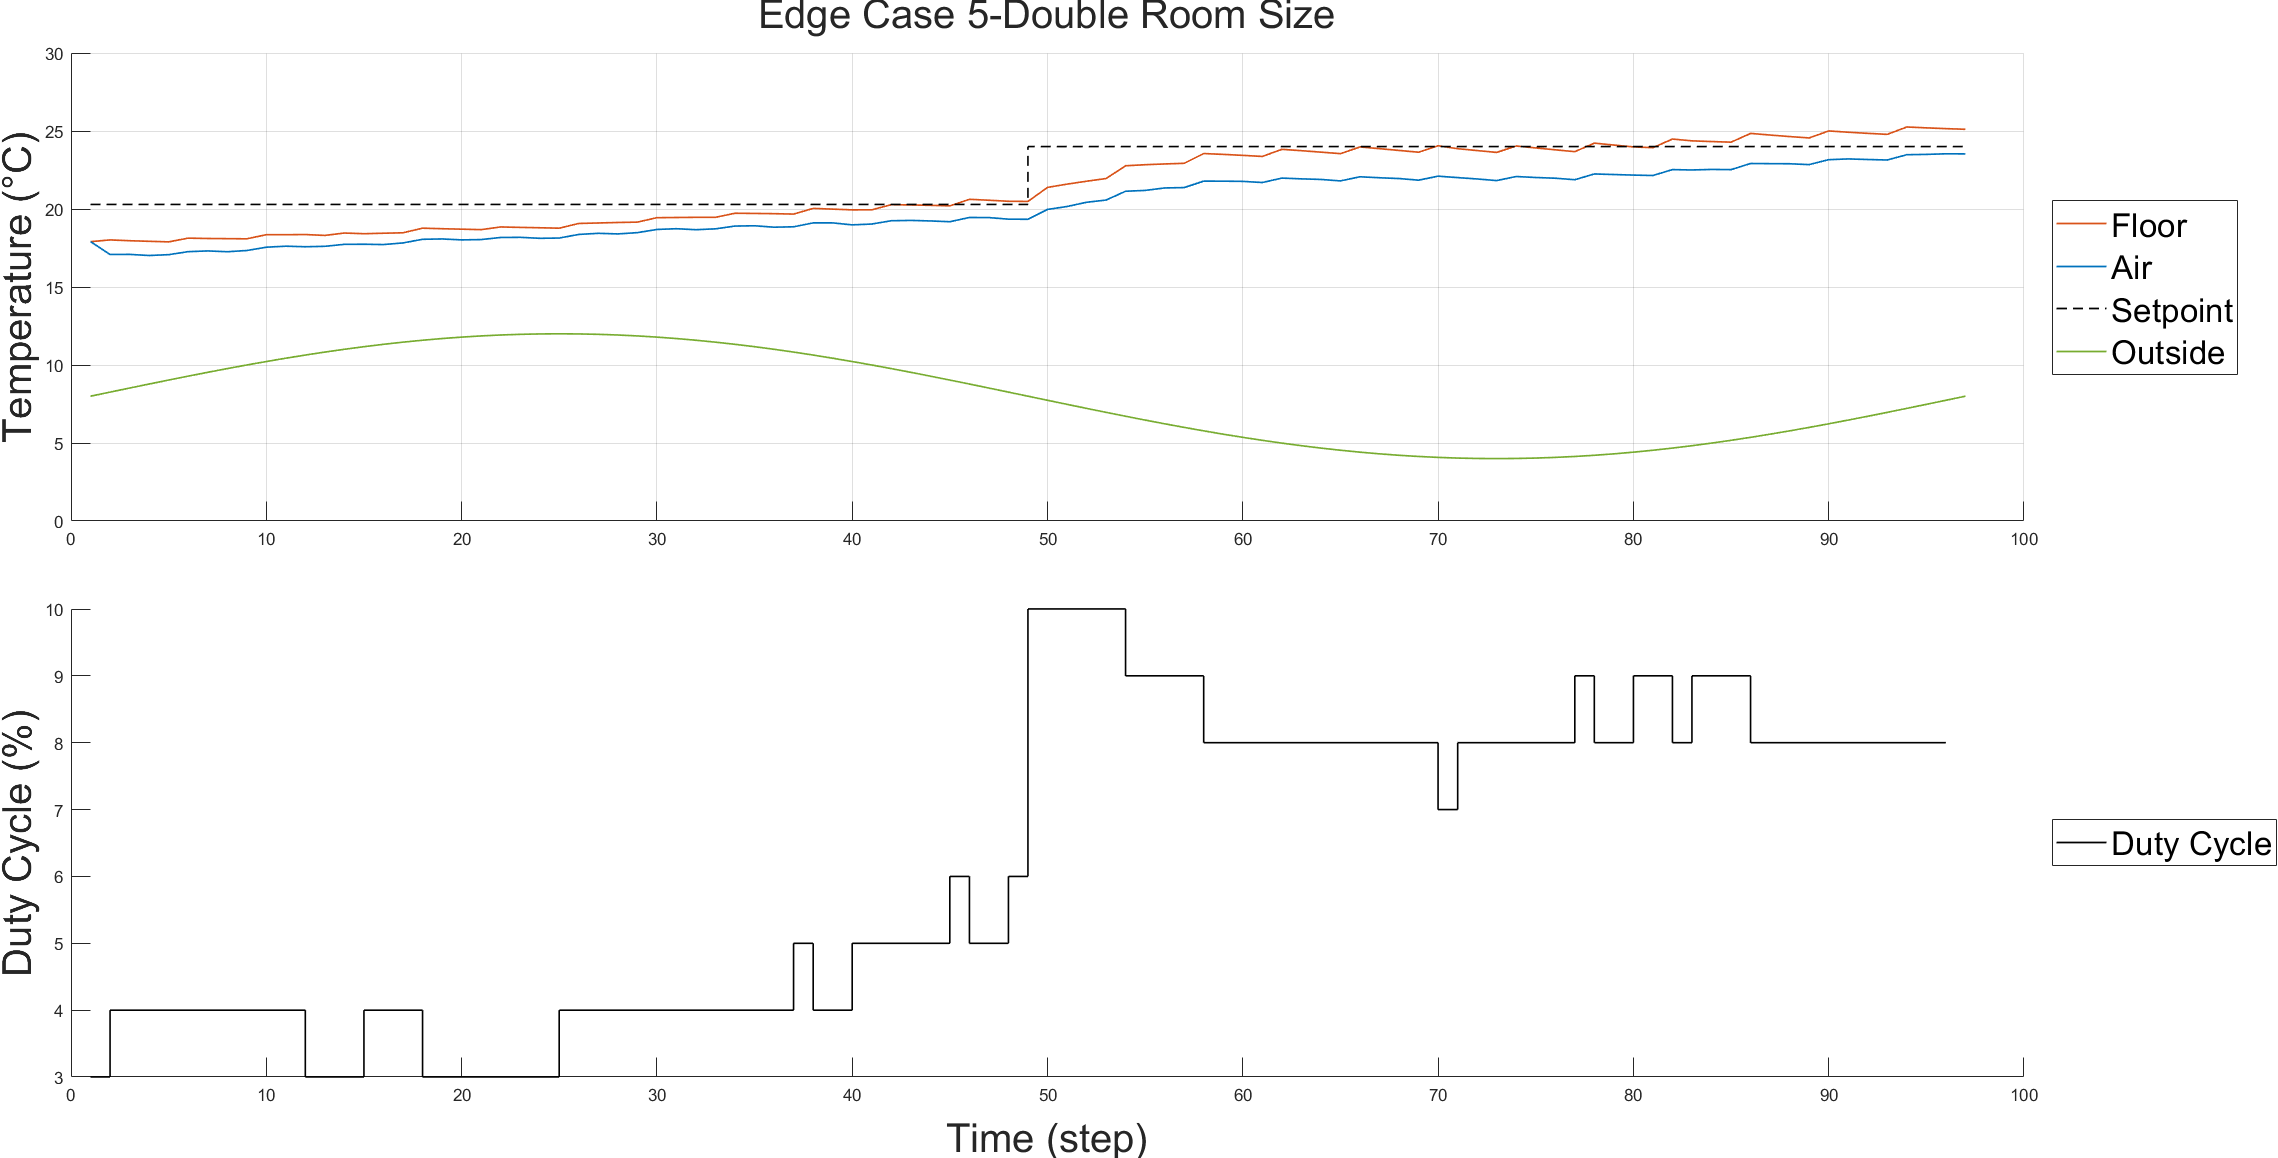
\includegraphics[width=1\linewidth]{figures/EdgeCase5-DoubleRoomSize.png}
        \caption{Doubled room with the same load}
        \label{fig:edge_5a}
    \end{subfigure}
    \begin{subfigure}{\textwidth}
    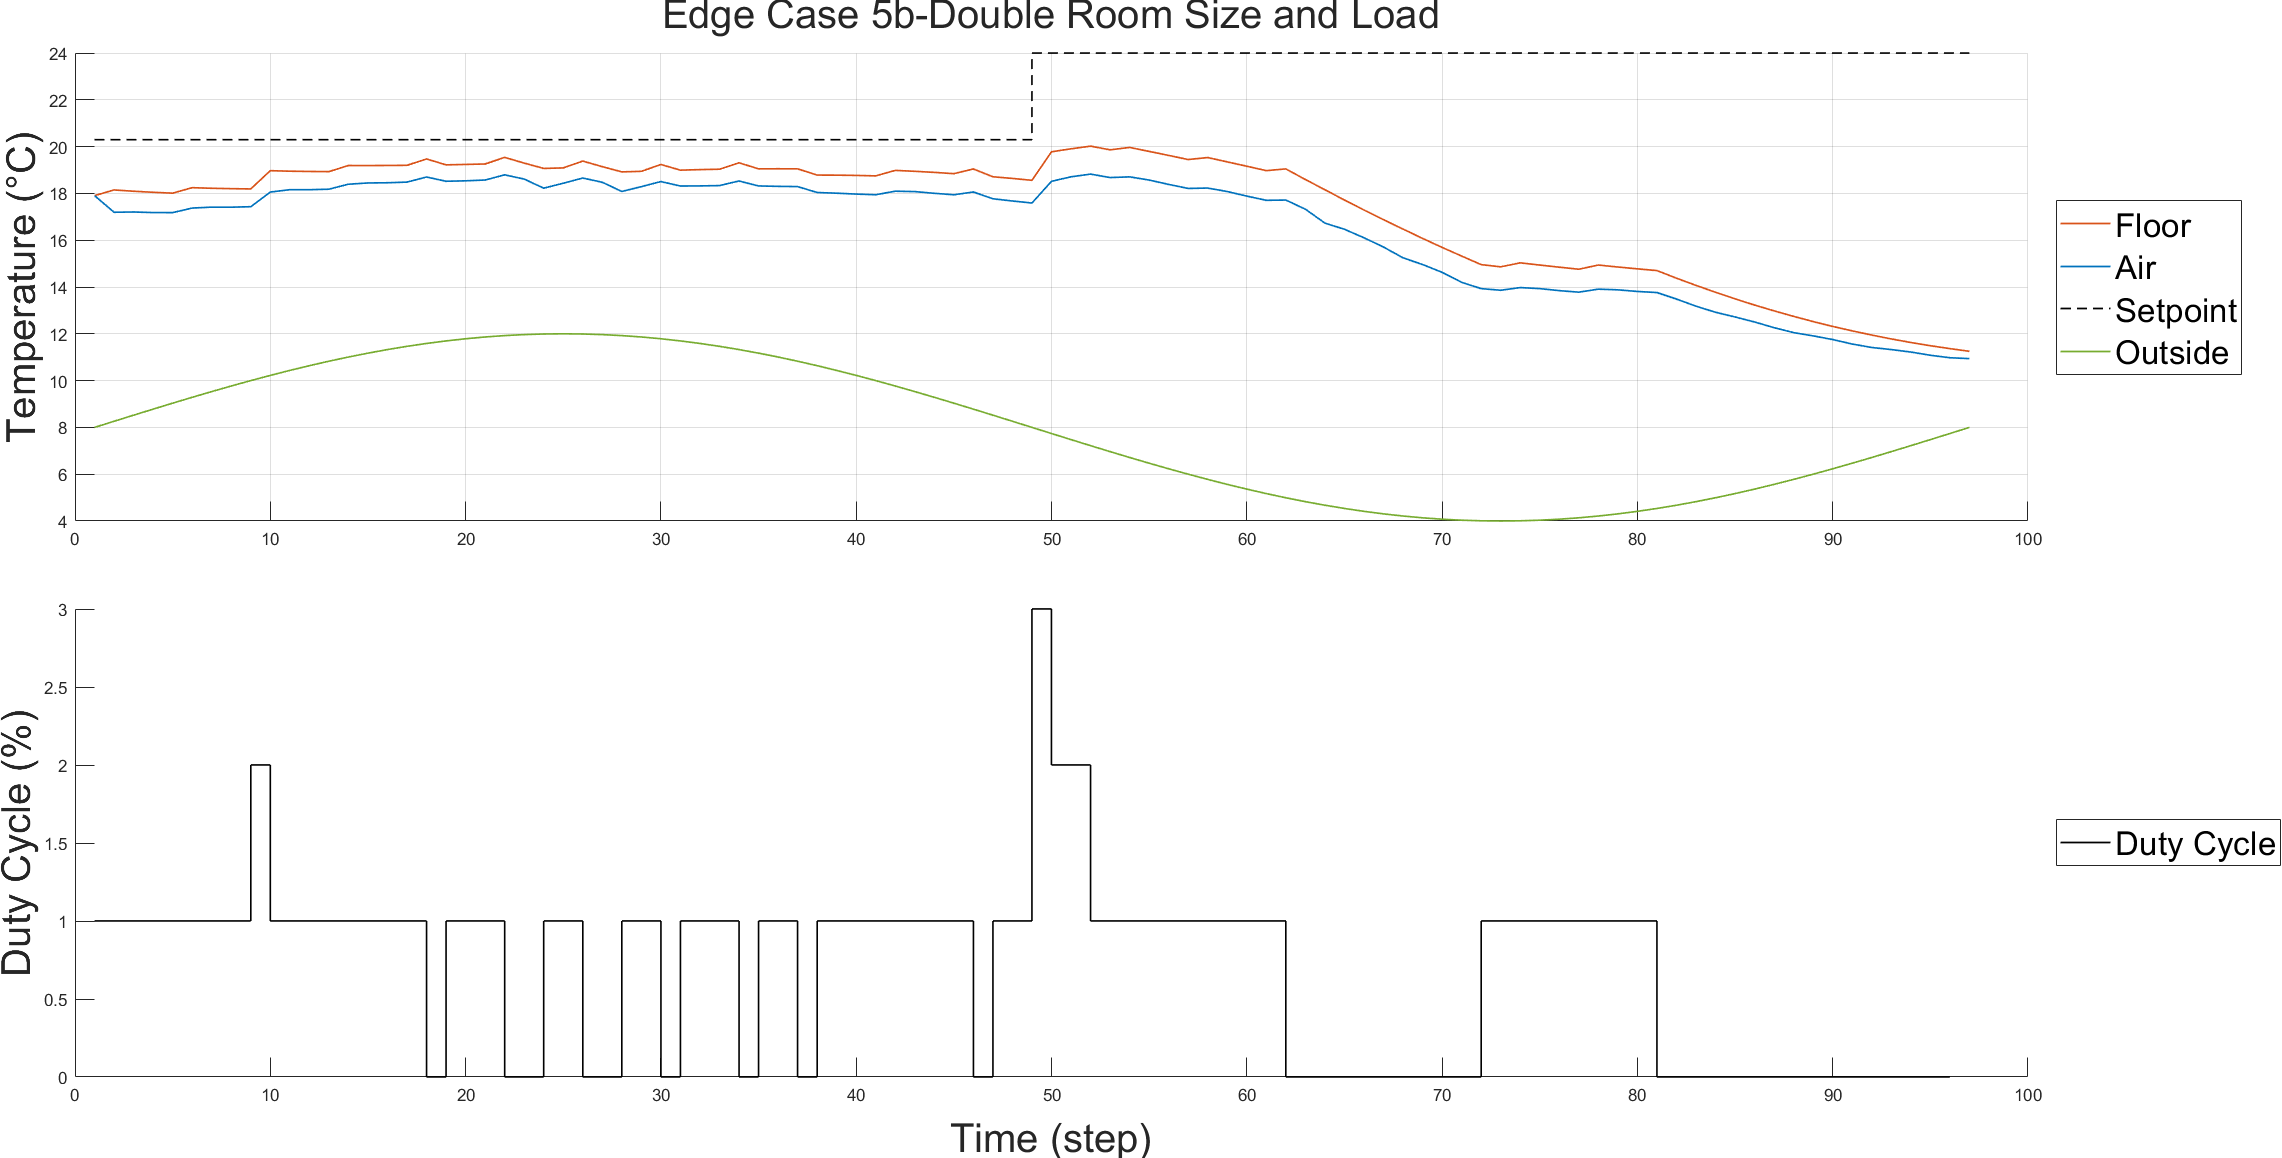
\includegraphics[width=1\linewidth]{figures/EdgeCase5b-DoubleRoomSizeandLoad.png}
    \caption{Doubled room with a doubled load}
    \label{fig:edge_5b}
    \end{subfigure}
\caption{Edge case 5: doubled room size}
\label{fig:edge_5}
\end{figure}

Note that a load of 2 (A) is sufficient for this room size as long as it turns on long enough. Yet, our algorithm cannot do so due to its lack of experience. A feasible solution is to create a new environment in which such cases exist so the agent can learn about them. Yet, continuous retraining may not suit all real-life situations. In short, a PI controller is better for this situation.


\section{OJ Benchmarks}
Table \ref{tab:uwg5_results} reveals the test results using computer simulation. Their configurations and formulas are exactly the same in section \ref{sec:env_baseline}. Note that the x-axes now display steps, not hours or seconds, in which
    $$1 \text{ step } = \tau_s = 15 \text{ (minutes)} $$
The average power cost in test case 2 remains the highest at 669.34 (kW), saving 8.62\% from a PI controller's 732.48 (kW). In case 1, our agent saves 7.13\% from 603.41 (kW) to 560.39 (kW), while in case 3, it cuts down to only 441.92 (kW), saving 6.59\%. The average number of relay switches is constant across all cases at five times per hour, which is only 0.26 times (case 3) and up to 1.89 (case 1) times fewer. The deviation of steady-state values about setpoints, on the other hand, is also improved though not very significant ($\pm 0.2$ (\degree C)); it still lies within the desired tolerance of $\pm 1$ (\degree C). The maximum overshooting and steady-state errors are also comparable to those of a PI controller, ranging from 0.82-1.1 (\degree C) and all zero, respectively.

\begin{table}[htbp]
\caption{UWG5 test configurations and results}
\label{tab:uwg5_results}
\centering
\begin{tabularx}{\textwidth}{|X|X|X|X|X|}
    \hline
    \textbf{Test no.} & \textbf{Test 1} (Fig. \ref{fig:result1}) & \textbf{Test 2} (Fig. \ref{fig:result2}) & \textbf{Test 3} (Fig. \ref{fig:result3}) \\
    \hline
    Load (A) & 10 & 15 & 15 \\
    \hline
    Outside temperature (°C)  & 17 & 17 & 12 \\
    \hline
    Initial value (°C) & 22.25 & 22.25 & 22.25 \\
    \hline \hline
    Deviation (°C) & $\pm 0.2$ & $\pm 0.2$ & $\pm 0.2$ \\
    \hline
    Max Overshoot (°C) & 0.95 & 0.82 & 1.10 \\
    \hline
    Avg. steady-state error (°C) & 0.00 & 0.00 & 0.00 \\
    \hline
    Power cost (kW) & 560.39 & 669.34 & 441.94 \\
    \hline
    Avg. relay switch (times/h) & 5.00 & 5.00 & 5.00 \\
    \hline
\end{tabularx}
\end{table}

\begin{figure}[htbp]
    \centering
    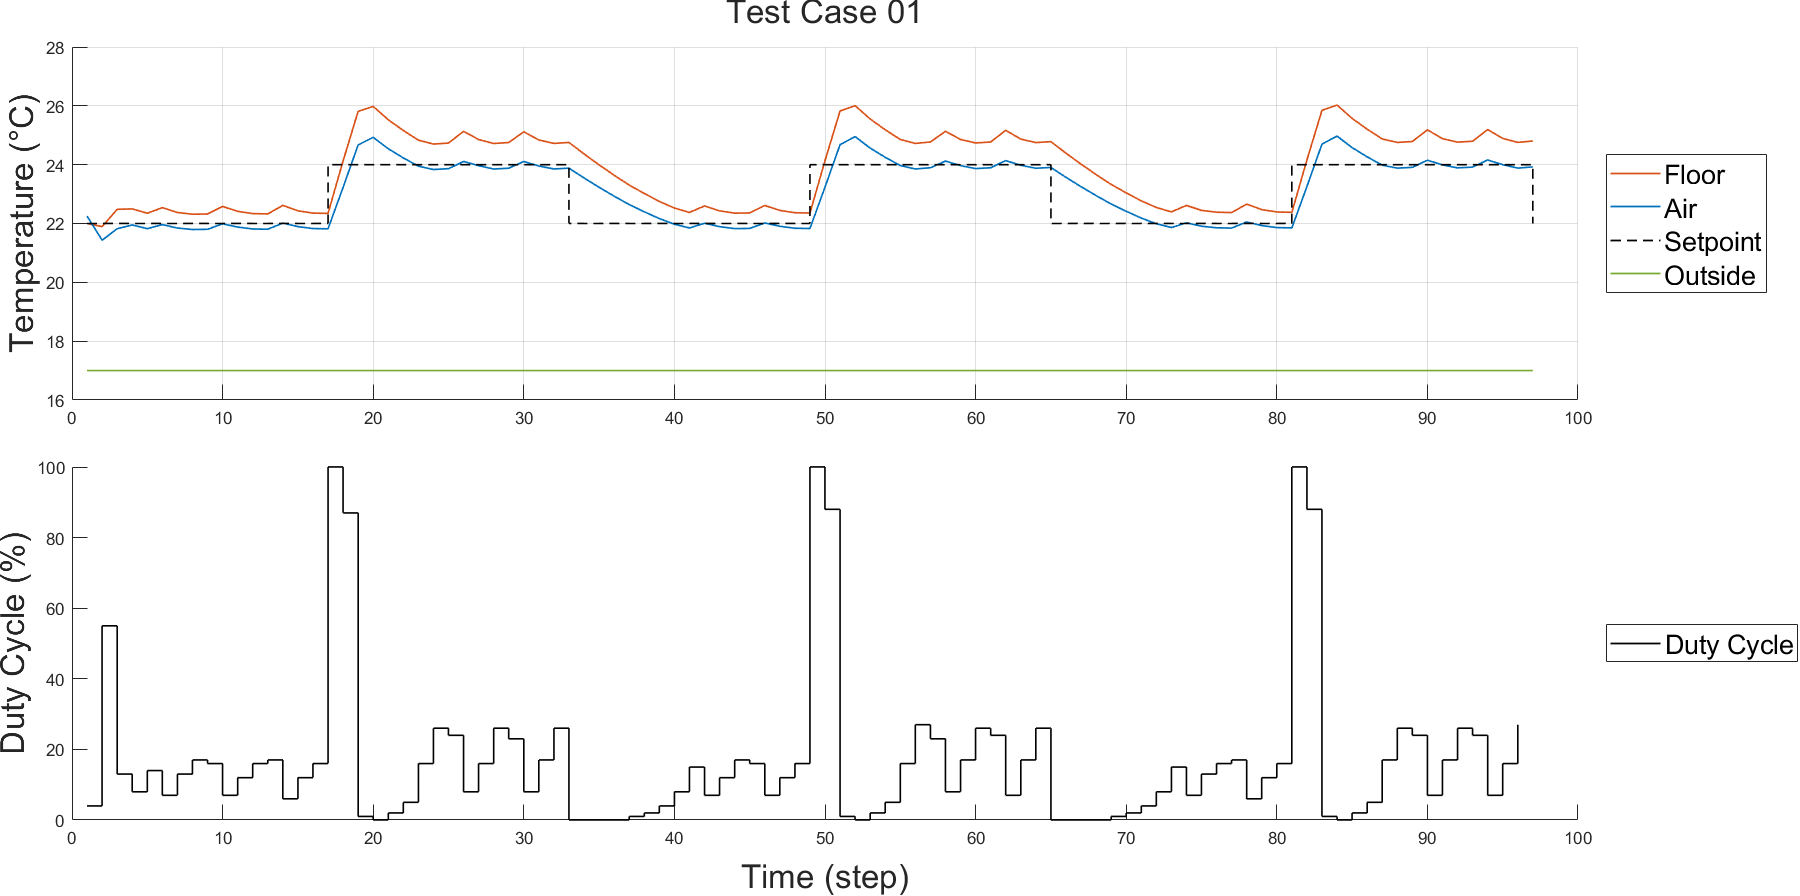
\includegraphics[width=1\linewidth]{figures/TestCase01.png}
    \caption{Benchmark of the best TD3 version on case 1}
    \label{fig:result1}
\end{figure}
\begin{figure}[htbp]
    \centering
    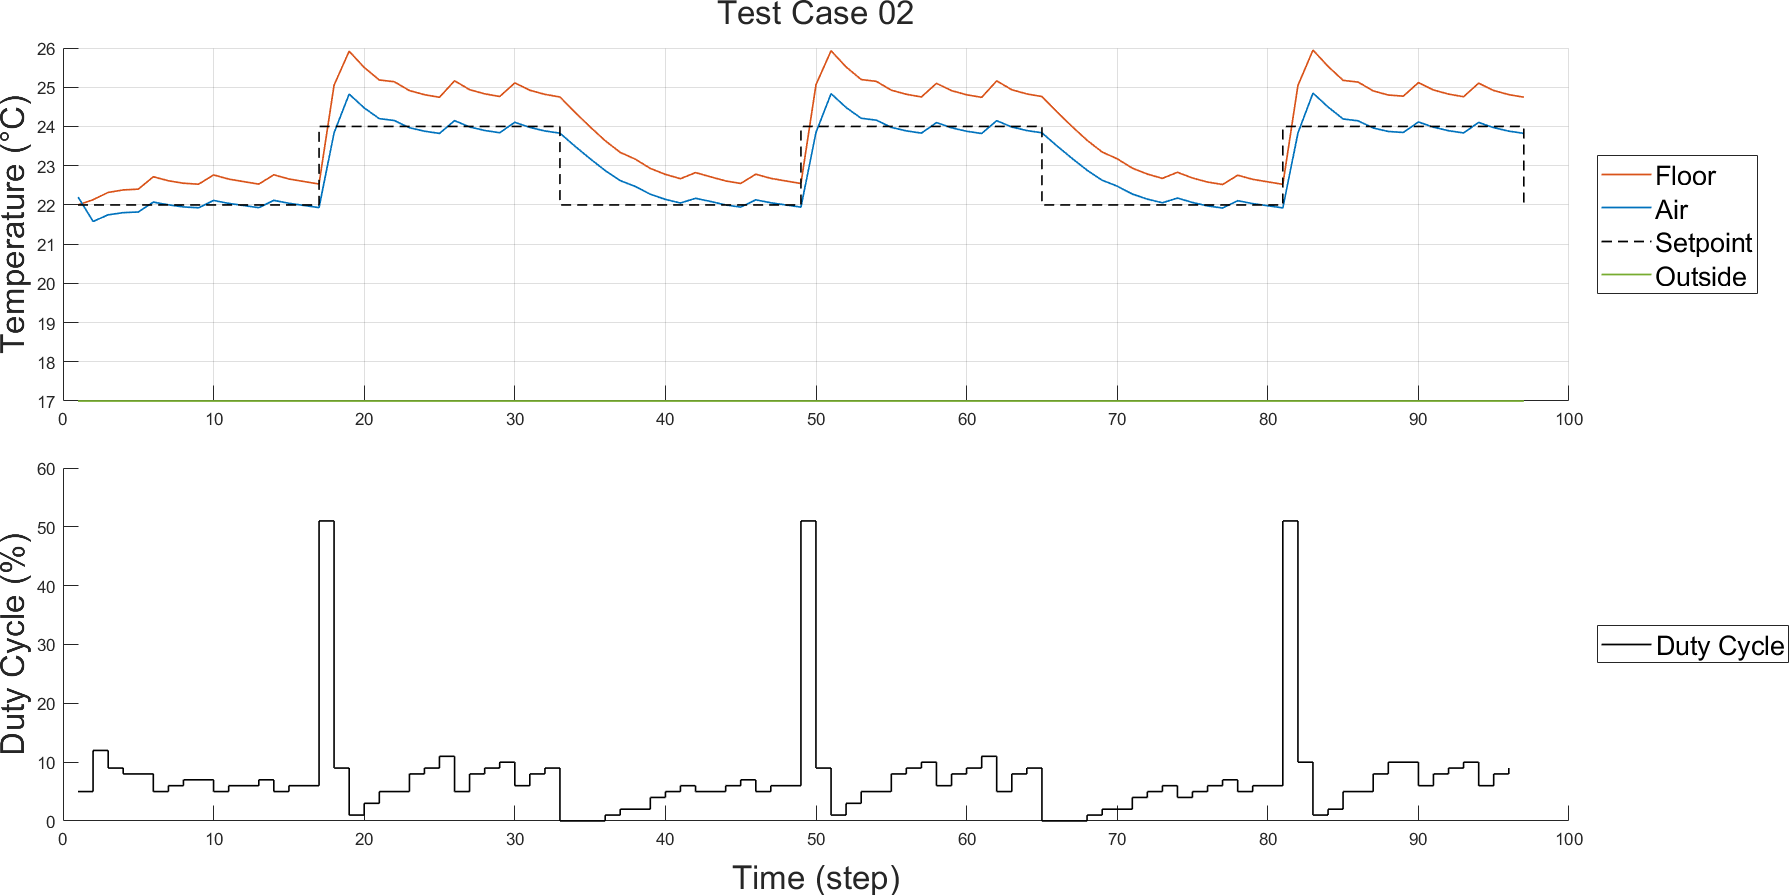
\includegraphics[width=1\linewidth]{figures/TestCase02.png}
    \caption{Benchmark of the best TD3 version on case 2}
    \label{fig:result2}
\end{figure}
\begin{figure}[htbp]
    \centering
    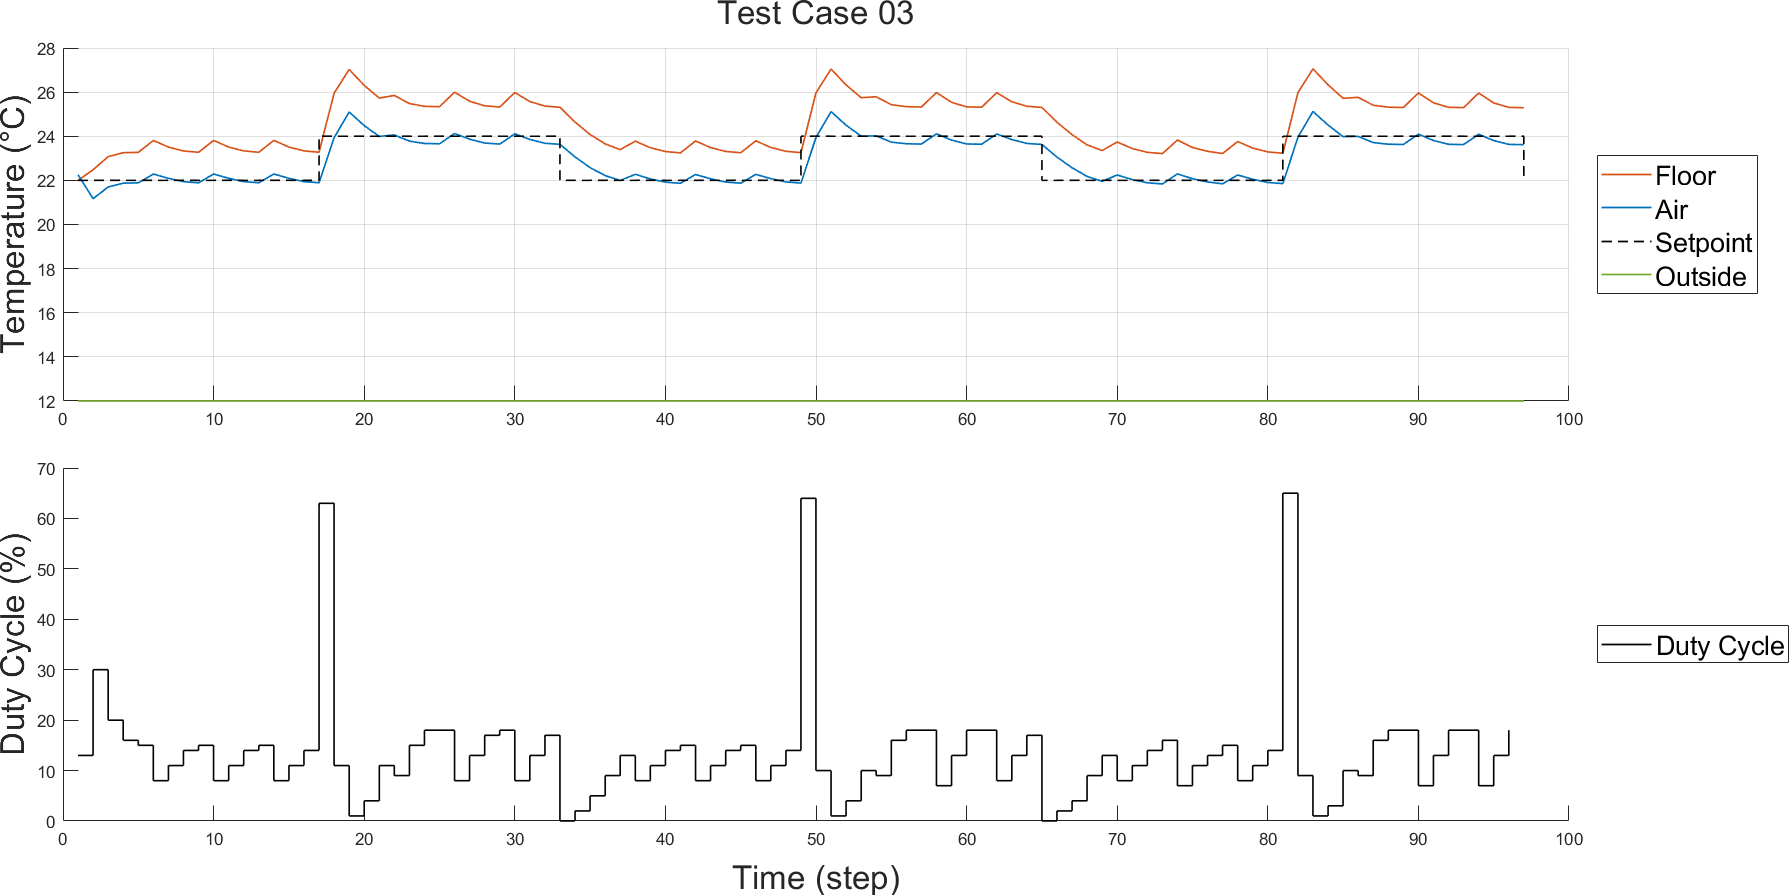
\includegraphics[width=1\linewidth]{figures/TestCase03.png}
    \caption{Benchmark of the best TD3 version on case 3}
    \label{fig:result3}
\end{figure}


\section{Conclusion}
This thesis thoroughly examines how reinforcement learning, specifically a model-free, online, off-policy agent like Twin-Delayed Deep Deterministic (TD3) Temporal Difference, can be built and applied to a relay-based thermostat for electrical floor heating through a series of the following tasks:
\begin{itemize}
    \item Record an actual system's data to construct a realistic thermodynamic model.
    \item Study similar research on reinforcement learning, especially its application to heating, ventilation, and air conditioning systems.
    \item Develop, train, and assess multiple experiments under various hyperparameters, reward functions, and edge cases.
\end{itemize}
Under three identical benchmarks, my proposal outperforms a traditional PI controller in most metrics with the best results as:
\begin{enumerate}
    \item 1.89 fewer relay switches per hour (test scenario 1)
    \item 8.62\% less energy consumption (test scenario 2)
    \item much smaller deviation about setpoints during stable time, i.e., only $\pm 0.2$ (\degree C) (all scenarios)
    \item comparable maximum overshooting of 0.82 (\degree C) (all scenarios)
    \item zero steady-state error of the average air temperature (all scenarios)
\end{enumerate}
Moreover, a TD3 algorithm is theoretically superior in three edge cases: when the outside temperature is higher, when the floor is nearly overheated, and when the air is much hotter due to immeasurable disturbances. In the case of natural cooling from a warm starting point, both controllers may have similar performance. In contrast, PI has the edge on intrinsic dynamical changes, which is also the most decisive score. This finding underscores that reliability and robustness are the biggest obstacles to bringing reinforcement learning to mass production. That is why we should not use reinforcement learning as a standalone replacement for existing PI/PID.


\section{Future Outlook}
The integration of reinforcement learning into thermodynamic control like underfloor heating holds significant promises:
\begin{enumerate}
    \item \textbf{High performance}: RL controllers can quickly adapt to changing conditions, learn from experience, and optimize their performance over time. Unlike traditional control methods, which rely on fixed parameters, RL can adjust dynamically based on real-time feedback.
   \item \textbf{Complex dynamics handling}: thermodynamic systems often exhibit nonlinearity, large delays, and complex behaviors. RL algorithms can handle these intricate dynamics by exploring control strategies and learning optimal policies.
   \item \textbf{Better user experience}: RL can significantly enhance user comfort by memorizing the usage patterns and personalizing the setpoints accordingly.
\end{enumerate}

Nevertheless, it still imposes many other challenges that we must fully tackle before commercializing, which are:
\begin{enumerate}
    \item \textbf{Safety} is paramount in any control system. RL controllers must be transparent and explainable to ensure trust and compliance. If the controller fails or behaves unexpectedly, it should seamlessly switch to a more interpretable method, such as PID control.
    \item \textbf{Explainability} is becoming a legal rule in many countries. Hence, interpretable RL schemes are essential to address these concerns. Techniques like SHAP (Shapley Additive Explanations) or LIME (Local Interpretable Model-agnostic Explanations) can help reveal the decision-making process.
    \item \textbf{Data dependency} is another hurdle of this approach. Training an effective model demands substantial data, which may not always be readily available in practical scenarios. Transfer learning, knowledge distillation, or human-in-the-loop are viable solutions we can investigate further.
    \item \textbf{Robustness} to system's changes such as building materials, weather conditions, room sizes, or user behaviors. Domain adaptation is a common technique that can mitigate this issue. So far, the simplest solution is to retrain the model continuously.
    \item \textbf{Fine-Tuning Complexity} Traditional PID controllers have only three parameters, making them relatively easy to fine-tune. In contrast, RL controllers have numerous hyperparameters and require careful tuning. Automated tuners such as Python's Optuna framework or meta-learning approaches can simplify this process.
\end{enumerate}

Lastly, the industry tends to favor established methods due to risk aversion. Convincing stakeholders to utilize RL requires clear advantages and zero safety concerns. Hence, more piloting projects with a balance between the strengths of RL and the reliability of traditional methods are necessary. With collaboration with academia, they can gradually build up the confidence for a wider adoption.

\end{document}